\section{Elementare Wahrscheinlichkeitsrechnung}
\label{sec:elementare-wahrscheinlichkeitsrechnung}
\subsection{Diskrete Wahrscheinlichkeitsräume}
\label{sec:diskrete-wahrscheinlichkeitsrume}
\subsubsection{Ergebnisraum}
\label{sec:definition}
Der \textbf{Ergebnisraum} $\Omega$ ist die Menge aller möglichen Ergebnisse des betrachteten Zufallsexperiments.
\subsubsection{Zähldichte}
\label{sec:zhl-dichte}
Die Zähldichte ist eine Funktion $p:\Omega \rightarrow \mathbb{R}$, die jedem Element aus $\Omega$ seine Wahrscheinlichkeit zuordnet.
Sie wird graphisch als Stabdiagramm dargestellt. Es gilt:
\begin{equation*}
    1 = \sum_{\omega \in \Omega} p(\omega)
\end{equation*}
\subsubsection{Ereignis}
Ein Ereignis ist eine Teilmenge von $\Omega$; der Ereignisraum $2^{\Omega}$ ist die Menge aller Teilmengen von $\Omega$.
\subsubsection{Diskretes Wahrscheinlichkeitsmass}
\label{sec:diskretes-wahrscheinlichkeitsmass}
Jede Zähldichte bestimmt ein diskretes Wahrscheinlichkeitsmass $P$. Dieses ordnet jedem Ereignis seine Wahrscheinlichkeit zu.
\begin{equation*}
    P: 2^{\Omega} \rightarrow [0,1],P(M) = \sum_{\omega \in M} p(\omega) \quad \forall M \subseteq \Omega
\end{equation*}
\subsubsection{Diskreter Wahrscheinlichkeitsraum}
\label{sec:diskreter-wahrscheinlichkeitsraum}
Der Ergebnisraum $\Omega$ versehen mit dem Wahrscheinlichkeitsmass $P$ heisst dann diskreter Wahrscheinlichkeitsraum und wird mit $\Omega ,P$ bezeichnet.
\subsection{Laplace-Raum}
\label{sec:laplace-raum}
Falls jedes Ergebnis aus $\Omega$ mit der gleich wahrscheinlich ist, wird $(\Omega ,P)$ ein \textbf{Laplace-Raum} genannt. Für diesen Fall gilt:
\begin{equation*}
    P(M) = \frac{|M|}{|\Omega|}
\end{equation*}
\subsection{Wichtige Eigenschaften diskreter Wahrscheinlichkeitsräume}
\label{sec:wichtige-eigenschaften-diskreter-wahrscheinlichkeitsrume}
\begin{itemize}
    \item Unmögliches Ereignis: $P(\emptyset) = 0$
    \item Sicheres Ereignis: $P(\Omega) = 1$
    \item Komplementäres Ereignis: $P(\Omega \setminus M) = 1 - P(M)$
    \item Vereinigung zweier Ereignisse: $P(M \cup N) = P(M) + P(N) - P(M \cap N)$
    \item Sigma-Additivität: $P(M_1 \cup M_2 \cup \dots \cup M_n) = P(A_1) + P(A_2) + \dots + P(A_n)$
        falls die Ereignisse $M_i$ paarweise disjunkt sind.
\end{itemize}
\subsection{Zufallsvariablen}
\label{sec:zufallsvariablen}
Sei $(\Omega ,P)$ ein diskreter Wahrscheinlichkeitsraum.
\subsubsection{Zufallsvariable}
\label{sec:zufallsvariable}
Jede Funktion $X:\Omega \rightarrow \mathbb{R}$, welche auf dem Ergebnisraum definiert ist und reelle Werte hat, heisst \textbf{Zufallsvariable}.
\subsubsection{Wahrscheinlichkeitsdichte}
\label{sec:wahrscheinlichkeitsdichte}
Die reelle Funktion $f:\mathbb{R} \rightarrow [0,1], f(x) = P(X = x)$ heisst \textbf{Wahrscheinlichkeitsdichte} oder kurz Dichtefunktion (PMF) von $X$.
\subsubsection{Kumuative Verteilungsfunktion}
\label{sec:kumuative-verteilungsfunktion}
Die reelle Funktion $F:\mathbb{R} \rightarrow [0,1], F(x) = P(X \leq x)$ heisst \textbf{Kumuative Verteilungsfunktion} (CDF) von $X$.
\subsection{Wichtige Eigenschaften von PMF und CDF}
\label{sec:wichtige-eigenschaften-von-pmf-und-cdf}
\begin{itemize}
    \item $\sum_{x=-\infty}^{\infty} f(x) = 1$ und $F(z)=\sum_{x=-\infty}^{z} f(x)$
    \item $\lim_{x \rightarrow \infty} F(x) = 1 und \lim_{x \rightarrow -\infty} F(x) = 0$
    \item Monotonie: Aus $x \leq y$ folgt $F(x) \leq F(y)$
    \item $f(x) = F(x) - \lim_{y \rightarrow x} F(y)$
    \item $P(a \leq X \leq b) = F(b) - F(a)$ und $P(a \leq X \leq b) = F(b) - \lim_{x \rightarrow a} F(x)$
    \item $P(X > b) = 1 - F(b)$ und $P(X \geq b) = 1 - \lim_{x \rightarrow b} F(x)$
\end{itemize}
\subsection{Kenngrössen}
\label{sec:kenngrssen}
Um Verteilungen vergleichen zu können bedient man sich einiger weniger charakteristischer Merkmale, sogenannter Kenngrössen. 
Wir betrachten Lagemasse und Streumasse. Lagemasse beschreiben das Zentrum der Verteilung und Streumasse charakterisieren die Abweichung vom Zentrum.
Seien $(\Omega, P)$ ein diskreter Wahrscheinlichkeitsraum und $X: \Omega \rightarrow \mathbb{R}$ eine Zufallsvariable.
\subsubsection{Erwartungswert}
\label{sec:erwartungswert}
Der Erwartungswert $E(X) = \sum_{x \in \mathbb{R}} P(X=x) \cdot y = \sum_{\omega \in \Omega} P(\left{\omega\right}) \cdot X(\omega)$ ist ein Lagemass der Verteilung von $X$.
Der Erwartungswert existiert nicht für jede Verteilung.
\subsubsection{Varianz}
\label{sec:varianz}
Die Varianz $V(X) = E(\left[X - E(X)\right]^2) = \sum_{x \in \mathbb{R}} P(X=x) \cdot \left[x - E(X)\right]^2
= \sum_{\omega \in \Omega} P(\left{\omega\right}) \cdot \left[X(\omega) - E(X)\right]^2$ und die Standardabweichung
$S(X) = \sqrt{V(X)}$ sind Streumassen der Verteilung von $X$. Varianz und Standardabweichung existieren nicht für jede Verteilung.
\subsection{Wichtige Eigenschaften der Kenngrössen}
\label{sec:wichtige-eigenschaften-der-kenngrssen}
\begin{itemize}
    \item Linearität: $E(X + Y) = E(X) + E(Y)$ und $E(\alpha X) = \alpha E(X)$, mit $\alpha X \in \mathbb{R}$
    \item Verschiebungssatz und die Varianz: $V(X) = E(X^2) - E(X)^2 = \left[\sum_{x \in \mathbb{R}} P(X=x) \cdot x^2\right] - E(X)^2$
    \item $V(\alpha X + \beta) = \alpha^2 V(X)$ mit $\alpha, \beta \in \mathbb{R}$
\end{itemize}
Im Allgemeinen gilt für die Verteilung einer Zufallsvariablen $X$ nach der Tschebyscheffschen Ungleichung, dass immer
mindestens 75\% der Werte im Bereich $E(X) \pm 2 \cdot S(X)$ liegen. \\
Viele Zufallsvariablen sind annähernd nach einer Gauss'schen Normalverteilung verteilt. Bei einer normalverteilten
Zufallsvariable liegen etwa 68\% der Werte im Bereich $E(X) \pm S(X)$ und bereits etwa 95\% im Bereich $E(X) \pm 2 \cdot S(X)$.
\subsection{Bedingte Wahrscheinlichkeiten}
\label{sec:bedingte-wahrscheinlichkeiten}
Seien $(\Omega, P)$ ein diskreter Wahrscheinlichkeitsraum und $A$ und $B$ zwei Ereignisse.
Die \textbf{bedingte Wahrscheinlichkeit} $P(A|B)$ ist die Wahrscheinlichkeit, dass Ereignis $A$ eintritt, unter der Annahme
dass Ereignis $B$ eingetreten ist. Falls $P(B) > 0$ ist, so gilt:
\begin{equation*}
    P(A|B) = \frac{P(A \cap B)}{P(B)}
\end{equation*}
\subsubsection{Wichtige Eigenschaften der bedingten Wahrscheinlichkeiten}
\label{sec:wichtige-eigenschaften-der-bedingten-wahrscheinlichkeiten}
\begin{itemize}
    \item Multiplikationssatz - Pfadwahrscheinlichkeit: $P(A \cap B) = P(A|B) \cdot P(B) = P(B|A) \cdot P(A)$
    \item Satz von der Totalen Wahrscheinlichkeit: $P(A) = P(A|B) \cdot P(B) + P(A|\overline{B}) \cdot P(\overline{B})$
        mit dem Komplement $\overline{B} = \Omega \setminus B$ von $B \subseteq \Omega$
    \item Satz von Bayes: $P(B|A) = \frac{P(B|A) \cdot P(A)}{P(B)}$
\end{itemize}
\begin{center}
    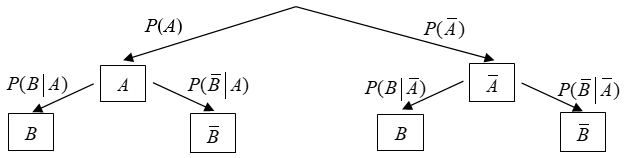
\includegraphics[width=1\textwidth]{images/Wahrscheinlichkeitsbaum.png}
\end{center}
\subsection{Stochastische Unabhängigkeit}
\label{sec:stochastische-unabhngigkeit}
Seien $(\Omega, P)$ ein diskreter Wahrscheinlichkeitsraum und $A$ und $B$ zwei Ereignisse.
Die Ereignisse $A$ und $B$ sind \textbf{stochastisch unabhängig}, falls gilt:
\begin{equation*}
    P(A \cap B) = P(A) \cdot P(B)
\end{equation*}
Andernfalls sind die Ereignisse \textbf{stochastisch abhängig}. \\
Zwei Zufallsvariablen $X: \Omega \rightarrow \mathbb{R}$ und $Y: \Omega \rightarrow \mathbb{R}$ 
heissen \textbf{stochastisch unabhängig}, falls gilt:
\begin{equation*}
    P(X=x, Y=y) = P(X=x) = P(X=x) \cdot P(Y=y) \quad \forall x, y \in \mathbb{R}
\end{equation*}
Andernfalls heissen die Zufallsvariablen \textbf{stochastisch abhängig}. \\
Die Funktion $f(x, y) = P(X=x, Y=y)$ heisst \textbf{gemeinsame Verteilung} (Verbundverteilung) von $X$ und $Y$.
\subsubsection{Satz von der stochastischen Unabhängigkeit}
\label{sec:satz-von-der-stochastischen-unabhngigkeit}
Sei $(\Omega, P)$ ein diskreter Wahrscheinlichkeitsraum. Folgende Eigenschaften sind äquivalent:
\begin{enumerate}
    \item $A$ und $B$ sind stochastisch unabhängig
    \item $A$ und $\Omega \setminus B$ sind stochastisch abhängig
    \item $B$ und $\Omega \setminus A$ sind stochastisch abhängig
    \item $\Omega \setminus A$ und $\Omega \setminus B$ sind stochastisch unabhängig
\end{enumerate}
Wenn $A$ und $B$ stochastisch unabhängig sind, beeinflusst das Eintreten des einen Ereignisses das Eintreten
des anderen Ereignisses nicht. \\
Denn falls $P(B) \neq 0$, so gilt $P(A|B) = P(A)$ und falls $P(A) \neq 0$, so gilt $P(B|A) = P(B)$. \\
Für stochastisch unabhängige Zufallsvariablen $X$ und $Y$ gilt:
\begin{equation*}
    E(X \cdot Y) = E(X) \cdot E(Y) \quad \text{und} \quad V(X + Y) = V(X) + V(Y)
\end{equation*}